\documentclass[12 pt, twoside]{article}
\input{../../mycommands}

%\addbibresource[datatype=bibtex]{../references.bib} % this command inputs the references file and analyzes it using bibtex
\begin{document}
\thetitle{Mathematics Review}[\sl For Applications In Physics]
\author{\EC}
\date{\today}
\fancyhf{}
\fancyhead[LE,RO]{\hyperlink{top}{\textbf{\thepage}}}
\fancyhead[LO,RE]{\small\sl\leftmark}
\setlength\headheight{17pt}

\pagenumbering{gobble} % no page number going forward!
\maketitle
\begingroup
    \parindent 0cm \parfillskip 0cm \leftskip 0cm \rightskip 0cm
    \etocframedstyle[1]{}
    \etocsetstyle{section}
                  {}
                  {} {\Large\bf\etocnumber.~\etocname\hfill\nobreak\tt p.~\makebox[12 pt][r]{\etocpage}\par}
                  {\vspace{-0.25cm}}
    \etocsetstyle{subsection}{}{}{}{}
    \etocsetstyle{subsubsection}{}{}{}{}
    \tableofcontents\label{toc:FirstPage}
\endgroup
\newpage
\subsection*{Statement of Purpose}
I am writing this as a review for myself of mathematial concepts that I have learned. I will not try and build from the ground up the concepts here. For example, I will just write about how to find the eigenvectors of a matrix, not how eigenvectors are defined. 
\subsubsection*{Notation I Like}  
    \begin{itemize}
    \item I try to stay as consistent as I can with variable and function letters; no one needs u {\sl and\/}~v for velocity. That being said, different fields do regularly use different notations, and it would be ridiculous of me to ignore them entirely, I'll try to include some ``translations'' for important things.
    \item
    I like Euler, Leibniz, Newton notation for differentiation. all of the following can be considered equivalent: 
    \begin{align*}
        \der{x}f&=\der{f}{x}=\der*{x}f=f'(x)
        \\
        \pder{x}f&=\pder{f}{x}=\pder*{x}f=f_x(x,y)
    \end{align*}
    \item Bold notation will be used over arrow notation for vectors.  
    \begin{equation*}
        \vb{A}= A_i=
        \begin{bmatrix}
        A_r
        \\
        A_\theta
        \\
        A_\phi
        \end{bmatrix} =A_r\e{r}+A_\theta\e{\theta}+A_\phi\e{\phi}
    \end{equation*}   
    \item A function $f$ is linear if you can take out constants and add/subtract without changing the function:\footnote{Examples of functions that aren't linear are: \(f(x)=\sin(x)\,,\,f(x)= x^2\)}
    \begin{align*}
        f(cx)&=cf(x)\quad c\in \mathbb{R}
        \\
        f(x\pm y)&=f(x)\pm f(y)
    \end{align*}
    \end{itemize}
\newpage\pagenumbering{arabic} % arabic page numbering going forward!
\endinput
\newpage
% Since \input doesn't like preambles, only uncomment next line if you're editing this TeX, don't forget the \end{document}!
%\documentclass{article}\usepackage[utf8]{inputenc} % allows for non-ASCII input characters like ä
\usepackage[x11names]{xcolor}% Color extensions, load first
\usepackage[margin=1in]{geometry} % Formatting on page
\usepackage{array} % better arrays
\usepackage{amsmath} % Math symbols and formats
    \numberwithin{equation}{section} % amsmath command that renews equation counter in each section\
\usepackage{amsthm}   
\usepackage{amssymb}
\usepackage[backend=bibtex]{biblatex} % bibliography
\usepackage{bm} % bold, even for greek letters
\usepackage{enumitem} % Enumerating things
\usepackage{esint} % better double and triple Integrals
\usepackage{etoc} % super powerful table of contents
\usepackage{fancyhdr} % Headers
    \pagestyle{fancy}
\usepackage{gensymb} % more symbols
\usepackage{physics} % easier commands for physics things
\usepackage{relsize}  % allows for larger/smaller math 
\usepackage{textcomp} % Gets rid of perthousand error
\usepackage{upquote}  % fixes quotes in verbatim environment
\usepackage{verbatim} % Allows for comment environment
\usepackage{tikz} % pictures and drawings
    \usetikzlibrary{calc}
    \usetikzlibrary{3d}
    %\usetikzlibrary{external}
    %\tikzexternalize
    %\tikzsetexternalprefix{figures/}
\usepackage{pgfplots} % plots and graphics
    \pgfplotsset{compat=newest} % or use compat=1.6 
\usepackage{graphicx} % plots and graphics
\usepackage{xparse} % Better commands
\usepackage[hidelinks]{hyperref}% References--THIS GOES LAST
\usepackage[utf8]{inputenc} % allows for non-ASCII characters
\usepackage[x11names]{xcolor}    % Color extensions
\usepackage[margin=1in]{geometry} % Formatting on page
\usepackage{array} % big arrays
\usepackage{amsmath} % Math symbols
\usepackage{amsthm}   
\usepackage{amssymb}
\usepackage[backend=bibtex]{biblatex} % bibliography
\usepackage{bm} % bold for greek letters
\usepackage{cancel}
\usepackage[format=hang]{caption}
\usepackage{enumitem} % Enumerating things
\usepackage{esint} % better double and triple Integrals
\usepackage{etoc}
\usepackage{fancyhdr} % Headers
    \pagestyle{fancy}
\usepackage{float}
\usepackage{gensymb}
\usepackage{physics} % easier commands for physics things
\usepackage{relsize}  % allows for larger/smaller math 
\usepackage{textcomp} % Gets rid of perthousand error
\usepackage{upquote}  % fixes quotes in verbatim environment
\usepackage{verbatim} % Allows for comment environment
\usepackage{tikz} % pictures
	\usetikzlibrary{calc}
	\usetikzlibrary{decorations.markings}
	\usetikzlibrary{3d}
	\usetikzlibrary{intersections}
\usepackage{pgfplots} % plots and graphics
	\pgfplotsset{compat=newest} % or use compat=1.6
	\usepgfplotslibrary{fillbetween}
\usepackage{graphicx} % plots and graphics
\usepackage{wrapfig}
\usepackage{xparse} % Better commands
\usepackage[hidelinks]{hyperref}% References--THIS GOES LAST

% Packages that this breaks without: amsmath, gensymb, physics, hyperref, xcolor, xparse, and possibly others
\numberwithin{equation}{section} % amsmath command that renews equation counter in each section\
\def\ints{\int_\mathcal{S}} % Surface integral
\def\intv{\int_\mathcal{V}} % Volume integral with V subscript
\def\intall{\int_{-\infty}^{\infty}} % Integral over all space
\def\iintall{\iint_{\rm All Space}} % Integral over all space
\def\iiintall{\iiint_{\rm All Space}} % Integral over all space
\def\ik{4\pi\epsilon_0} % Inverse k for EM
\def\lap{\mathcal{L}}
\def\answerline{ % double horizontal line placed 0.5 cm below text, space between lines is 0.07 cm, then 0.75 cm of space 
	\vspace{0.5 cm}
	\hrule
	\vspace{0.07 cm}
	\hrule
	\vspace{0.75 cm}\noindent} % don't indent text after the line
\NewDocumentCommand\length{O{3pt}}{\setlength\jot{#1}} % for align vertical spacing, there's probably a better way to do this locally
\NewDocumentCommand\ft{s O{n} O{L}}{ % I dont want to write \sin(stuff) \cos(stuff) every time in fourier transforms (ft)
    \IfBooleanTF{#1}{
        \sin(\frac{#2 \pi}{#3}x)
    }{
        \cos(\frac{#2 \pi}{#3}x)
    }
}

\NewDocumentCommand\dl{s}{\IfBooleanTF{#1}{}{\cdot} d\mathbf{l}} % quicker curve integral dl, if no star, it also makes the dot 
\NewDocumentCommand\da{s}{\IfBooleanTF{#1}{}{\cdot} d\mathbf{a}} % quicker surface integral da, if no star, it also makes the dot 
\NewDocumentCommand\oo{O{1} m} {\frac{#1}{#2}}   % reciprocal- 'one over', option to make it a regular fraction because oo is still quicker to type.
\NewDocumentCommand\thetitle{m O{}}{ \title{ \hypertarget{top}{\textbf{#1}} \\ \large {#2} } } %Bold title that is a hypertarget, optional bolded subtitle that's scaled properly 

\NewDocumentCommand \e {s m}{ % basis vector command
	\IfBooleanTF{#1} % \e{x} for x hat notation, \e*{x} for e_x notation
	{\mathbf{\hat{e}_{#2}}}
	{\bm{\hat{#2}}}} % from package bm, more powerful than \mathbf} 
\NewDocumentCommand \parametric {m}{ %command for getting boundary conditions with a "{" on the left
    \left\{ 
	\begin{gathered}
		\begin{matrix}
			#1
    		\end{matrix}
	\end{gathered}
	 \right.}
\NewDocumentCommand \der {s O{} m g}{ % custom derivative command
     \IfBooleanTF{#1} % if \der*, #1 is true, euler notation used, if \der , #1 is false, d/dx is used 
    {\IfNoValueTF{#4}  % g returns -NoValue- if no argument (read below)
        {\mathrm{D}_{#3}^{#2}}  % g is included so \der{x} and \der{f}{x} both have x in the denominator
        {\mathrm{D}_{#4}^{#2}#3}
            }
    {\IfNoValueTF{#4}
        {\frac{\mathrm{d}^{#2}}{\mathrm{d} #3^{#2}}}
        {\frac{\mathrm{d}^{#2} #3}{\mathrm{d} #4^{#2}}}
	}}    
\NewDocumentCommand \pder {s O{} m g}{ % custom partial derivative command, allows for euler notation if starred
     \IfBooleanTF{#1}
        {\IfNoValueTF{#4}
            {\partial_{#3}^{#2}}
            {\partial_{#4}^{#2}#3}
                }
        {\IfNoValueTF{#4}
            {\frac{\partial^{#2}}{\partial #3^{#2}}}
            {\frac{\partial^{#2} #3}{\partial #4^{#2}}}
                }} 
                
\NewDocumentCommand \header {m m m}{
	\fancyhead[L]{#1} 
	\fancyhead[C]{\hyperlink{top}{ \textbf{#2} }}
	\fancyhead[R]{#3}
	\fancyfoot[C]{--\thepage--}
	\pagestyle{fancy}
	\setlength\headheight{17pt}}
    
\NewDocumentCommand{\coloredanswer}{O{LavenderBlush2} m}{ % makes coloredbox with pretty color
	\mathchoice
	{\colorbox{#1}{$\displaystyle #2$}}
	{\colorbox{#1}{$\textstyle #2$}}
	{}
	{}}

\newcounter{probcount} % new counter for problem numbers, starts at 0 by default
\NewDocumentEnvironment{ problem } {O{} +b} %Problem environment for homework, autocounts numbers, behaves like a section and can get listed (and hyperlinked) in the toc. 
	{\addtocounter{probcount}{1} % increase counter at the beginning of every problem
	 \phantomsection % invisible page marker for hyperref
	 \addcontentsline{toc}{subsection}{Problem \theprobcount. {\it#1}} % add "Problem \theprobcount. \textit{#1}" to table of contents (toc) as if it were a subsection
	 \begin{trivlist} % begin unmarked ("trivial") list
	 \item {\bf Problem \theprobcount.} {\it#1} % print Problem with the counter and optional text 
	 \item #2  % +b is for inputs that are long
	 \end{trivlist} % end list
	}{} % don't do anything then "problem" environment ends, irrelevant because trivlist is already ended
	
\def\UM{\colorbox{blue}{\textcolor{Gold1}{\textbf{University of Michigan}}}} % School Pride
\def\EC{\href{https://github.com/CarpenterEvan/PhysicsReview}{\(\mathbb{E}\textsc{van}~\mathbb{C}\textsc{arpenter}\)}}
\endinput\begin{document}
\section{Differential Calculus}
    \subsection*{Differentiation in One Dimension (1-D)}
        The derivative is the proportionality factor of how rapidly the function \(f(x)\) varies when the argument \(x\) is changed by \(dx\); \(f\) changes by an amount \(df\):
        \begin{align*}
            df = \qty(\der{f}{x})dx
        \end{align*}
        Multiplying and dividing functions $f=f(x),~g=g(x)$, in derivatives 
        \\
        Product Rule:
        \begin{equation}
            \der{x}(fg)=(f')g+f(g')
        \end{equation}
        Quotient Rule:
        \begin{equation}
            \der{x}\qty(\frac{f}{g})=\frac{(f')g-f(g')}{{(g)}^2}
        \end{equation}
    \subsection*{Differentiation in Three Dimensions (3-D)}
        For 3-variable functions:
        \begin{align*}
            df =\qty(\der{f}{x})dx + \qty(\der{f}{y})dy + \qty(\der{f}{z})dz
        \end{align*}
        The derivative of \(f(x,y,z)\) tells one how \(f\) changes when one alters all three variables by \(dx, dy, dz\).
    \subsection*{Gradient}
        \begin{align*}
            \grad f(x,y,z) = 
            \begin{bmatrix}
                \pder*{x}
                \\
                \pder*{y}
                \\
                \pder*{z}
            \end{bmatrix}
            f(x,y,z) = \coloredanswer{\pder{f}{x}\e{x}+\pder{f}{y}\e{y}+\pder{f}{z}\e{z}}
        \end{align*}
        The del operator ($\nabla$) is a \textcolor{Blue1}{\bf vector derivative operator}. It can take in a scalar field $f(x,y,z)$ and returns a vector field. The vectors \textcolor{Blue1}{\bf points in the direction of \(f\)'s maximum increase of the scalar field}, moreover, the magnitude of \(\nabla f\) gives the magnitude of each vector along this maximal direction.
        \\[0.5 cm]
        Just like 1-D derivatives, you can find the extrema of a function with three variables by observing it at a stationary point \((x,y,z)\):
        \begin{align*}
            \nabla f = 0 
        \end{align*}
        Gradients obey the following product rules:
        \begin{gather*}
            \nabla (fg) = (\nabla f)g + f (\nabla g) 
            \\
            \nabla (\vb{A} \cdot \vb{B}) 
            = (\vb{A} \cdot \nabla)\vb{B} + (\vb{B} \cdot \nabla)\vb{A}+ \vb{A} \times (\nabla \times \vb{B}) + \vb{B} \times(\nabla \times \vb{A}) \\
        \end{gather*}
    \subsection*{Divergence}
        Divergence is a measure of how much a vector field spreads out from a point or volume.   The divergence of a vector field \(\vb{A}\) is caluclated by taking a dot product between the del operator and a \(\vb{A}\). \textcolor{Blue1}{\bf The divergence of a vector field is a scalar.} 
        \begin{equation}
            \div\vb{A}=
            \qty[
                \begin{matrix}
                    \pder*{x}\\\pder*{y}\\\pder*{z}
                \end{matrix}
            ]\cdot\qty[
                \begin{matrix}
                    A_x\\A_y\\A_z
                \end{matrix}
            ]=
            \coloredanswer{\pder{A_x}{x}+\pder{A_y}{y}+\pder{A_z}{z}}
        \end{equation}
        Divergences obey the following Product Rules:
        {\length[0.25 cm]
        \begin{align*}
            \div(f\vb{A}) &= f(\nabla \cdot \vb{A}) + \vb{A} \cdot (\nabla f)
            \\
            \div{(\vb{A} \times \vb{B})} &= \vb{B} \cdot (\nabla \times \vb{A}) - \vb{A} \cdot (\nabla \times \vb{B})
        \end{align*}
        }
        When the divergence of a vector field is zero everywhere it is called {\bf solenoidal}. Any closed surface has no net flux across it in a solenoidal field.
    \subsection*{Curl}
        Curl is a measure of how much a vector ``swirls'' around the point in question. The curl of a vector field \(\vb{A}\) is found by taking the cross product of the del operator with \(\vb{A}\). One can find the curl conveniently as the determinant of the following matrix: 
        \begin{equation}
            \curl \vb{A} = 
            \qty[
                \begin{matrix}
                    \pder*{x}\\\pder*{y}\\\pder*{z}
                \end{matrix}
            ]\cross\qty[
                \begin{matrix}
                    A_x\\A_y\\A_z
                \end{matrix}
            ]=
            \begin{vmatrix}
            \e{x}&\e{y}&\e{z}
            \\
            \pder*{x}&\pder*{y}&\pder*{z}
            \\
            A_x&A_y&A_z
            \end{vmatrix}
            =\coloredanswer{
            \begin{bmatrix}
            (\pder*{y} A_z-\pder*{z} A_y)
            \\[0.25 cm]
            (\pder*{z} A_x-\pder*{x} A_z)
            \\[0.25 cm]
            (\pder*{x} A_y-\pder*{y} A_x)
            \end{bmatrix}
            \cdot
            \begin{bmatrix}
            \e{x}
            \\
            \e{y}
            \\
            \e{z}
            \end{bmatrix}}
        \end{equation}
        Curls obey the following Product Rules:
        \begin{align*}
        \curl (f\vb{A}) &= f(\curl \vb{A}) - \vb{A} \times (\nabla f)
        \\[0.3 cm]
        \curl (\vb{A} \times \vb{B}) &= (\vb{B} \cdot \nabla)\vb{A} - (\vb{A} \cdot \nabla)\vb{B} + \vb{A}(\nabla \cdot \vb{B}) - \vb{B}(\nabla \cdot \vb{A})
        \end{align*}
        \textcolor{Blue1}{\bf The curl of a vector field is a vector field.}\footnote{\sl Technically\rm\ a pseudo-vector field.} When the curl of a vector field is zero, the field is called {\bf irrotational} and the field is conservative. %(See Section \textbf{\ref{vectorfields}})
    \subsection*{Laplacian}
        The laplace operator (denoted by \(\nabla^2\)) is a kind of second derivative for scalars and vectors.\footnote{Some people use \(\Delta\) instead of \(\nabla^2\), but that seems goofy, so I don't use it.} It can be thought of as taking whichever vector derivatives are possible. 
        \begin{align}
            \nabla^2f
            &=\nabla \cdot (\nabla f)
            \\
            \nabla^2 \vb{A} 
            &= \nabla(\nabla \cdot \vb{A}) - \nabla\times (\nabla \times \vb{A}) 
        \end{align}
        The following is also true for second derivatives based on the nature of first order vector derivatives:
        \begin{gather}
            \nabla\times (\nabla f)
            = 0
            \\
            \nabla \cdot (\nabla \times \vb{A}) 
            = 0 
        \end{gather}
\newpage
\section{Integral Calculus}      
    Remember that \(\dl*,~\da*,\) and $dV$ are different in different coordinate systems.
    \length[0.5 cm]
    \begin{align}
        \textbf{ \large Curve Integral}&
        \quad\int_C \vb{A}\dl=\iiint\vb{A}\cdot\qty(dx\ \e{x}+dy\ \e{y}+dz\ \e{z})
        \\
        \textbf{\large Surface Integral}&\quad
        \int_S \vb{A}\da=\iint_D(\vb{A}\cdot\e{z})dxdy=\iint_D A_k dx_idx_j
        \\
        \textbf{\large Volume Integral}&\quad
        \int_{\mathcal{V}} \vb{A} dV=\int A_xdV\ \e{x}+\int A_ydV\ \e{y}+\int A_z dV\ \e{z}
    \end{align}
    \length

    \subsection*{The Fundamental Theorem for Gradients}
        Similar to the fundamental theorem of calculus, the curve integral of the gradient of a scalar function is equal to the difference of values of that scalar function at the endpoints. 
        \begin{equation}
            \boxed{\int_C(\nabla f)\dl=f(\mathbf{b})-f(\mathbf{a})}
        \end{equation}
    \subsection*{Divergence Theorem}
        The divergence of \(\vb{A}\) over a volume is equal to the components of \(\vb{A}\) that are normal to the surface that bounds the volume.\footnote{\(\oint\) is the closed path/closed surface integral sign.}
        \begin{align}
            \boxed{\oint_S \vb{A} \da =\int_{\mathcal{V}} (\nabla \cdot \vb{A})dV } 
        \end{align}
    \subsection*{The Fundamental Theorem for Curls: Stokes' Theorem}
        The integral of a derivative over a region is equal to the value of the function at the boundary. That is, the curl over a surface is equal to the value of the function at the perimeter P. 
        \begin{align}
            \boxed{\oint_C \vb{A} \cdot d\vb{l}=\int_{S} (\nabla \times \vb{A}) \cdot d\vb{a}} 
        \end{align}
        \subsection*{Integration by Parts in Vector Calculus}
        \begin{align*}
        \int_{\mathcal{V}} f(\nabla \cdot \vb{A})dV = \oint_S f\vb{A}\da-\int_{\mathcal{V}} \vb{A} \cdot (\nabla f)dV 
        \end{align*}


        \newpage


\section{Theories with Vector Fields \label{vectorfields}}
    \subsubsection*{The Helmholtz Theorem}
        A field is uniquely determined by its divergence and curl when boundary conditions are applied. If there exists a scalar field \(\phi\), and vector field \(\vb{A}\), \(C\), and:
        This means that a vector field \(\vb{F}\) can be :
        \begin{equation}
            \vb{F}=-\nabla V+\curl\vb{A}
        \end{equation}
        \begin{align*}
            \left.
            \begin{gathered}
            \nabla \cdot \vb{A}= \phi
            \\
            \nabla \times \vb{A}= \vb{C}
            \end{gathered}
            \right\}
            \implies
            \nabla \cdot \vb{C} = 0
        \end{align*}
        Then \(\vb{A}\) can be determined uniquely from $\phi$ and $\vb{C}$
    \subsubsection*{Potentials}
        If the curl of a vector field $\vb{E}$ vanishes everywhere, then the field is conservative, meaning that the curve integral between any two points is path independent (so if the path is closed, the curve integral is zero) and by definition of conservative fields, $\vb{E}$ can be represented as the gradient of some scalar function $V$:
        \footnote{The negative of the gradient is \textbf{used by convention} to make physics easier. Think about the gravitational force compared to gravitational potential, the force field points from from high (scalar) potential to low (scalar) potential.}
        \begin{align*}
            \boxed{\nabla \times \vb{E} = 0} 
            \iff
            \boxed{\oint_C \vb{E}\cdot d\vb{l}=0} 
            \iff
            \boxed{\vb{E} = -\nabla V}
        \end{align*}

        If the divergence of a vector field, $\vb{B}$, vanishes everywhere, then the surface integral of $\vb{B}$ is independent of the surface for any given boundary line. 
        \begin{align*}
            \boxed{\nabla \cdot \vb{B} = 0} 
            \iff
            \boxed{\oint_S\vb{B}\cdot d\vb{s}=0}
            \iff
            \boxed{\vb{B} = \nabla \times \vb{A}}
        \end{align*}
        
%\end{document}
\newpage
\section{Maxwell-Heaviside Equations}
\begin{align*}
	\div\vb{E}&=\frac{\rho}{\epsilon_0}
	&
	\oiint_{S}\vb{E}\da&=\iiint_{\mathcal{V}}\rho\d V\tag{Gauss' Law}
	\\[0.25cm]
	\curl\vb{E}&=-\pdv{\vb{B}}{t}
	&
	\oint_{C}\vb{E}\dl&=-\pdv{t}\iint_{S}\vb{B}\da\tag{Maxwell-Faraday Equation}
	\\[0.25cm]
	\div\vb{B}&=0
	&
	\oiint_{S}\vb{B}\da&=0\tag{Gauss' Law}
	\\[0.25cm]
	\curl\vb{B}&=\mu_0\vb{J}
	&
	\oint_{C}\vb{B}\dl&=\mu_0\iint_{S}\vb{J}\da\tag{Ampere's Law}
	\\
	&+\epsilon_0\mu_0\pdv{\vb{E}}{t}&&+\epsilon_0\mu_0\iint_{S}\pdv{\vb{E}}{t}\da\tag{Maxwell's Correction}
\end{align*}
\section{Fields in Matter}
Fields inside media that are not vaccuum:
\section{Retarded Potentials}
\begin{align*}
	\vb{E}(\vb{x},t)&=\frac{q}{4\pi\epsilon_0}\qty{\qty[\oo{\gamma^2}\frac{\vb{R}-R\vb*{\beta}}{\qty(R-\vb*{\beta}\cdot\vb{R})^3}]_\text{ret}
	+\qty[\oo{c^2}\frac{\vb{R}\cross\qty[\qty(\vb{R}-R\vb*{\beta})\cross\vb{a}]}{\qty(R-\vb{R}\cdot\vb*{\beta})^3}]_\text{ret}}
\end{align*}
With:
\begin{align*}
	\gamma&=\qty(1-\vb*{\beta}^2)
	&
	\vb*{\beta}&=\frac{\vb{v}}{c}
	\\
	\vb{R}&=\vb{x}-\vb{x}_0(\tau_0)
\end{align*}

\newpage
% Since \input doesn't like preambles, only uncomment next line if you're editing this TeX, don't forget the \end{document}! 
%\documentclass{article}\usepackage[utf8]{inputenc} % allows for non-ASCII characters
\usepackage[x11names]{xcolor}    % Color extensions
\usepackage[margin=1in]{geometry} % Formatting on page
\usepackage{array} % big arrays
\usepackage{amsmath} % Math symbols
\usepackage{amsthm}   
\usepackage{amssymb}
\usepackage[backend=bibtex]{biblatex} % bibliography
\usepackage{bm} % bold for greek letters
\usepackage{cancel}
\usepackage[format=hang]{caption}
\usepackage{enumitem} % Enumerating things
\usepackage{esint} % better double and triple Integrals
\usepackage{etoc}
\usepackage{fancyhdr} % Headers
    \pagestyle{fancy}
\usepackage{float}
\usepackage{gensymb}
\usepackage{physics} % easier commands for physics things
\usepackage{relsize}  % allows for larger/smaller math 
\usepackage{textcomp} % Gets rid of perthousand error
\usepackage{upquote}  % fixes quotes in verbatim environment
\usepackage{verbatim} % Allows for comment environment
\usepackage{tikz} % pictures
	\usetikzlibrary{calc}
	\usetikzlibrary{decorations.markings}
	\usetikzlibrary{3d}
	\usetikzlibrary{intersections}
\usepackage{pgfplots} % plots and graphics
	\pgfplotsset{compat=newest} % or use compat=1.6
	\usepgfplotslibrary{fillbetween}
\usepackage{graphicx} % plots and graphics
\usepackage{wrapfig}
\usepackage{xparse} % Better commands
\usepackage[hidelinks]{hyperref}% References--THIS GOES LAST

% Packages that this breaks without: amsmath, gensymb, physics, hyperref, xcolor, xparse, and possibly others
\numberwithin{equation}{section} % amsmath command that renews equation counter in each section\
\def\ints{\int_\mathcal{S}} % Surface integral
\def\intv{\int_\mathcal{V}} % Volume integral with V subscript
\def\intall{\int_{-\infty}^{\infty}} % Integral over all space
\def\iintall{\iint_{\rm All Space}} % Integral over all space
\def\iiintall{\iiint_{\rm All Space}} % Integral over all space
\def\ik{4\pi\epsilon_0} % Inverse k for EM
\def\lap{\mathcal{L}}
\def\answerline{ % double horizontal line placed 0.5 cm below text, space between lines is 0.07 cm, then 0.75 cm of space 
	\vspace{0.5 cm}
	\hrule
	\vspace{0.07 cm}
	\hrule
	\vspace{0.75 cm}\noindent} % don't indent text after the line
\NewDocumentCommand\length{O{3pt}}{\setlength\jot{#1}} % for align vertical spacing, there's probably a better way to do this locally
\NewDocumentCommand\ft{s O{n} O{L}}{ % I dont want to write \sin(stuff) \cos(stuff) every time in fourier transforms (ft)
    \IfBooleanTF{#1}{
        \sin(\frac{#2 \pi}{#3}x)
    }{
        \cos(\frac{#2 \pi}{#3}x)
    }
}

\NewDocumentCommand\dl{s}{\IfBooleanTF{#1}{}{\cdot} d\mathbf{l}} % quicker curve integral dl, if no star, it also makes the dot 
\NewDocumentCommand\da{s}{\IfBooleanTF{#1}{}{\cdot} d\mathbf{a}} % quicker surface integral da, if no star, it also makes the dot 
\NewDocumentCommand\oo{O{1} m} {\frac{#1}{#2}}   % reciprocal- 'one over', option to make it a regular fraction because oo is still quicker to type.
\NewDocumentCommand\thetitle{m O{}}{ \title{ \hypertarget{top}{\textbf{#1}} \\ \large {#2} } } %Bold title that is a hypertarget, optional bolded subtitle that's scaled properly 

\NewDocumentCommand \e {s m}{ % basis vector command
	\IfBooleanTF{#1} % \e{x} for x hat notation, \e*{x} for e_x notation
	{\mathbf{\hat{e}_{#2}}}
	{\bm{\hat{#2}}}} % from package bm, more powerful than \mathbf} 
\NewDocumentCommand \parametric {m}{ %command for getting boundary conditions with a "{" on the left
    \left\{ 
	\begin{gathered}
		\begin{matrix}
			#1
    		\end{matrix}
	\end{gathered}
	 \right.}
\NewDocumentCommand \der {s O{} m g}{ % custom derivative command
     \IfBooleanTF{#1} % if \der*, #1 is true, euler notation used, if \der , #1 is false, d/dx is used 
    {\IfNoValueTF{#4}  % g returns -NoValue- if no argument (read below)
        {\mathrm{D}_{#3}^{#2}}  % g is included so \der{x} and \der{f}{x} both have x in the denominator
        {\mathrm{D}_{#4}^{#2}#3}
            }
    {\IfNoValueTF{#4}
        {\frac{\mathrm{d}^{#2}}{\mathrm{d} #3^{#2}}}
        {\frac{\mathrm{d}^{#2} #3}{\mathrm{d} #4^{#2}}}
	}}    
\NewDocumentCommand \pder {s O{} m g}{ % custom partial derivative command, allows for euler notation if starred
     \IfBooleanTF{#1}
        {\IfNoValueTF{#4}
            {\partial_{#3}^{#2}}
            {\partial_{#4}^{#2}#3}
                }
        {\IfNoValueTF{#4}
            {\frac{\partial^{#2}}{\partial #3^{#2}}}
            {\frac{\partial^{#2} #3}{\partial #4^{#2}}}
                }} 
                
\NewDocumentCommand \header {m m m}{
	\fancyhead[L]{#1} 
	\fancyhead[C]{\hyperlink{top}{ \textbf{#2} }}
	\fancyhead[R]{#3}
	\fancyfoot[C]{--\thepage--}
	\pagestyle{fancy}
	\setlength\headheight{17pt}}
    
\NewDocumentCommand{\coloredanswer}{O{LavenderBlush2} m}{ % makes coloredbox with pretty color
	\mathchoice
	{\colorbox{#1}{$\displaystyle #2$}}
	{\colorbox{#1}{$\textstyle #2$}}
	{}
	{}}

\newcounter{probcount} % new counter for problem numbers, starts at 0 by default
\NewDocumentEnvironment{ problem } {O{} +b} %Problem environment for homework, autocounts numbers, behaves like a section and can get listed (and hyperlinked) in the toc. 
	{\addtocounter{probcount}{1} % increase counter at the beginning of every problem
	 \phantomsection % invisible page marker for hyperref
	 \addcontentsline{toc}{subsection}{Problem \theprobcount. {\it#1}} % add "Problem \theprobcount. \textit{#1}" to table of contents (toc) as if it were a subsection
	 \begin{trivlist} % begin unmarked ("trivial") list
	 \item {\bf Problem \theprobcount.} {\it#1} % print Problem with the counter and optional text 
	 \item #2  % +b is for inputs that are long
	 \end{trivlist} % end list
	}{} % don't do anything then "problem" environment ends, irrelevant because trivlist is already ended
	
\def\UM{\colorbox{blue}{\textcolor{Gold1}{\textbf{University of Michigan}}}} % School Pride
\def\EC{\href{https://github.com/CarpenterEvan/PhysicsReview}{\(\mathbb{E}\textsc{van}~\mathbb{C}\textsc{arpenter}\)}}
\endinput\begin{document}
\section{Linear Algebra}
\subsection{Eigenvalue, Eigenvector, Eigenfunction}
By definition an eigenvector $\vb{v}$ of a matrix $\vb{M}$ must satisfy: 
    \[\vb{M}\vb{v}=\lambda\vb{v}\quad\exists\lambda\in\mathbb{C}\]
    Rearranging to find $\lambda$ gives
    \begin{equation*}
        \vb{M}\vb{v}-\lambda\vb{v}=(\vb{M}-\lambda\vb{I})\vb{v}=0
    \end{equation*}
    The eigenvector $\vb{v}=0$ is a trivial solution, but if the matrix $(\vb{M}-\lambda\vb{I})$ is invertible, then it's inverse can be applied to both sides, leaving us with no choice but $\vb{v}=0$. Because of this, nontrivial values of $\lambda$ are therefore values that make $(\vb{M}-\lambda\vb{I})$ singular (i.e. non-invertible). 
    A matrix is singular if the determinant is zero, so to find nontrivial $\lambda$, you solve: 
    \begin{equation*}
        \det(\vb{M}-\lambda\vb{I})=\qty|\vb{M}-\lambda\vb{I}|=0
    \end{equation*}
%\end{document}
\newpage
% Since \input doesn't like preambles, only uncomment next line if you're editing this TeX, don't forget the \end{document}! 
%\documentclass{article}\usepackage[utf8]{inputenc} % allows for non-ASCII characters
\usepackage[x11names]{xcolor}    % Color extensions
\usepackage[margin=1in]{geometry} % Formatting on page
\usepackage{array} % big arrays
\usepackage{amsmath} % Math symbols
\usepackage{amsthm}   
\usepackage{amssymb}
\usepackage[backend=bibtex]{biblatex} % bibliography
\usepackage{bm} % bold for greek letters
\usepackage{cancel}
\usepackage[format=hang]{caption}
\usepackage{enumitem} % Enumerating things
\usepackage{esint} % better double and triple Integrals
\usepackage{etoc}
\usepackage{fancyhdr} % Headers
    \pagestyle{fancy}
\usepackage{float}
\usepackage{gensymb}
\usepackage{physics} % easier commands for physics things
\usepackage{relsize}  % allows for larger/smaller math 
\usepackage{textcomp} % Gets rid of perthousand error
\usepackage{upquote}  % fixes quotes in verbatim environment
\usepackage{verbatim} % Allows for comment environment
\usepackage{tikz} % pictures
	\usetikzlibrary{calc}
	\usetikzlibrary{decorations.markings}
	\usetikzlibrary{3d}
	\usetikzlibrary{intersections}
\usepackage{pgfplots} % plots and graphics
	\pgfplotsset{compat=newest} % or use compat=1.6
	\usepgfplotslibrary{fillbetween}
\usepackage{graphicx} % plots and graphics
\usepackage{wrapfig}
\usepackage{xparse} % Better commands
\usepackage[hidelinks]{hyperref}% References--THIS GOES LAST

% Packages that this breaks without: amsmath, gensymb, physics, hyperref, xcolor, xparse, and possibly others
\numberwithin{equation}{section} % amsmath command that renews equation counter in each section\
\def\ints{\int_\mathcal{S}} % Surface integral
\def\intv{\int_\mathcal{V}} % Volume integral with V subscript
\def\intall{\int_{-\infty}^{\infty}} % Integral over all space
\def\iintall{\iint_{\rm All Space}} % Integral over all space
\def\iiintall{\iiint_{\rm All Space}} % Integral over all space
\def\ik{4\pi\epsilon_0} % Inverse k for EM
\def\lap{\mathcal{L}}
\def\answerline{ % double horizontal line placed 0.5 cm below text, space between lines is 0.07 cm, then 0.75 cm of space 
	\vspace{0.5 cm}
	\hrule
	\vspace{0.07 cm}
	\hrule
	\vspace{0.75 cm}\noindent} % don't indent text after the line
\NewDocumentCommand\length{O{3pt}}{\setlength\jot{#1}} % for align vertical spacing, there's probably a better way to do this locally
\NewDocumentCommand\ft{s O{n} O{L}}{ % I dont want to write \sin(stuff) \cos(stuff) every time in fourier transforms (ft)
    \IfBooleanTF{#1}{
        \sin(\frac{#2 \pi}{#3}x)
    }{
        \cos(\frac{#2 \pi}{#3}x)
    }
}

\NewDocumentCommand\dl{s}{\IfBooleanTF{#1}{}{\cdot} d\mathbf{l}} % quicker curve integral dl, if no star, it also makes the dot 
\NewDocumentCommand\da{s}{\IfBooleanTF{#1}{}{\cdot} d\mathbf{a}} % quicker surface integral da, if no star, it also makes the dot 
\NewDocumentCommand\oo{O{1} m} {\frac{#1}{#2}}   % reciprocal- 'one over', option to make it a regular fraction because oo is still quicker to type.
\NewDocumentCommand\thetitle{m O{}}{ \title{ \hypertarget{top}{\textbf{#1}} \\ \large {#2} } } %Bold title that is a hypertarget, optional bolded subtitle that's scaled properly 

\NewDocumentCommand \e {s m}{ % basis vector command
	\IfBooleanTF{#1} % \e{x} for x hat notation, \e*{x} for e_x notation
	{\mathbf{\hat{e}_{#2}}}
	{\bm{\hat{#2}}}} % from package bm, more powerful than \mathbf} 
\NewDocumentCommand \parametric {m}{ %command for getting boundary conditions with a "{" on the left
    \left\{ 
	\begin{gathered}
		\begin{matrix}
			#1
    		\end{matrix}
	\end{gathered}
	 \right.}
\NewDocumentCommand \der {s O{} m g}{ % custom derivative command
     \IfBooleanTF{#1} % if \der*, #1 is true, euler notation used, if \der , #1 is false, d/dx is used 
    {\IfNoValueTF{#4}  % g returns -NoValue- if no argument (read below)
        {\mathrm{D}_{#3}^{#2}}  % g is included so \der{x} and \der{f}{x} both have x in the denominator
        {\mathrm{D}_{#4}^{#2}#3}
            }
    {\IfNoValueTF{#4}
        {\frac{\mathrm{d}^{#2}}{\mathrm{d} #3^{#2}}}
        {\frac{\mathrm{d}^{#2} #3}{\mathrm{d} #4^{#2}}}
	}}    
\NewDocumentCommand \pder {s O{} m g}{ % custom partial derivative command, allows for euler notation if starred
     \IfBooleanTF{#1}
        {\IfNoValueTF{#4}
            {\partial_{#3}^{#2}}
            {\partial_{#4}^{#2}#3}
                }
        {\IfNoValueTF{#4}
            {\frac{\partial^{#2}}{\partial #3^{#2}}}
            {\frac{\partial^{#2} #3}{\partial #4^{#2}}}
                }} 
                
\NewDocumentCommand \header {m m m}{
	\fancyhead[L]{#1} 
	\fancyhead[C]{\hyperlink{top}{ \textbf{#2} }}
	\fancyhead[R]{#3}
	\fancyfoot[C]{--\thepage--}
	\pagestyle{fancy}
	\setlength\headheight{17pt}}
    
\NewDocumentCommand{\coloredanswer}{O{LavenderBlush2} m}{ % makes coloredbox with pretty color
	\mathchoice
	{\colorbox{#1}{$\displaystyle #2$}}
	{\colorbox{#1}{$\textstyle #2$}}
	{}
	{}}

\newcounter{probcount} % new counter for problem numbers, starts at 0 by default
\NewDocumentEnvironment{ problem } {O{} +b} %Problem environment for homework, autocounts numbers, behaves like a section and can get listed (and hyperlinked) in the toc. 
	{\addtocounter{probcount}{1} % increase counter at the beginning of every problem
	 \phantomsection % invisible page marker for hyperref
	 \addcontentsline{toc}{subsection}{Problem \theprobcount. {\it#1}} % add "Problem \theprobcount. \textit{#1}" to table of contents (toc) as if it were a subsection
	 \begin{trivlist} % begin unmarked ("trivial") list
	 \item {\bf Problem \theprobcount.} {\it#1} % print Problem with the counter and optional text 
	 \item #2  % +b is for inputs that are long
	 \end{trivlist} % end list
	}{} % don't do anything then "problem" environment ends, irrelevant because trivlist is already ended
	
\def\UM{\colorbox{blue}{\textcolor{Gold1}{\textbf{University of Michigan}}}} % School Pride
\def\EC{\href{https://github.com/CarpenterEvan/PhysicsReview}{\(\mathbb{E}\textsc{van}~\mathbb{C}\textsc{arpenter}\)}}
\endinput\begin{document}
\section{Curvilinear Coordinates}
\subsection{Spherical Coordinates}
    In this system of coordinates, the following describe the space's basis set:
    %\tikzsetnextfilename{spherical}
    \tikzfading[name=ball, outer color=transparent!50, inner color=transparent!100]
    \begin{figure}[H]
        \begin{tikzpicture}
            \draw [dotted] (2.3,0,2)--(2.3,2.3,2)--(0,2.3,0); % projection of r onto z and x axis
            \draw [orange!30, fill=orange!30] (0,0,0)--(0.75,0.75,0) arc [start angle=45, end angle=90,radius=10 mm] node at (0.25,0.7) [black] {$\theta$}; % Theta arc
            \begin{scope}[canvas is xz plane at y=0]
                \draw [dotted] (0,0)--(2.3,2);
                \fill [blue!20] (0,0)--(1.2,1) arc [start angle=45, end angle=120,radius=10 mm] node at (0.35,0.65) [black] {$\phi$};
            \end{scope}


            %\fill [path fading=ball, color=black] (0.07,0) circle (2.5);
            \draw [ultra thick, -latex] (0,0,0)--(3,0,0) node [anchor=north west] {\textbf{y}};
            \draw [ultra thick, -latex] (0,0,0)--(0,3,0) node [anchor=south]      {\textbf{z}};
            \draw [ultra thick, -latex] (0,0,0)--(0,0,3) node [anchor=north west] {\textbf{x}};


            \draw [ultra thick, blue!20, -latex] (2.3,2.3,2)--(3,2,0.7) node [anchor=west, color=black] {$\e{\phi}$}; 
            \draw [ultra thick, orange!30, -latex] (2.3,2.3,2)--(3,1.6,2.25) node [anchor= north, color=black] {$\e{\theta}$}; 
            \draw [ultra thick, blue, -latex] (2.3,2.3,2)--(3,3,2) node [anchor=south east, color=black] {$\e{r}$}; 
            \draw [ultra thick, red, -latex] (0,0,0)--(2.3,2.3,2) node at (1,0.5) {\textbf{r}};


            \node (description text) at (6,2,0) {Distance from the origin: r};
            \node at (description text.south) [xshift=29.5, yshift=-5] {Polar angle: $\theta$};
            \node at (description text.south) [xshift=19, yshift=-16] {Azimuthal angle: $\phi$};
        \end{tikzpicture}
    \end{figure}
    Important relationships:
    \begin{align*}
        \begin{bmatrix}
        \e{r}\\
        \e{\theta}\\
        \e{\phi}
        \end{bmatrix}
        &=
        \begin{bmatrix}
        \sin(\theta)\cos(\phi)&\sin(\theta)\sin(\phi)&\cos(\theta)\\
        \cos(\theta)\cos(\phi)&\cos(\theta)\sin(\phi)&-\sin(\theta)\\
        -\sin(\phi)&\cos(\phi)&0
        \end{bmatrix}
        \begin{bmatrix}
        \e{x}\\
        \e{y}\\
        \e{z}
        \end{bmatrix}
    \end{align*}
    \begin{center}
    Matrix is orthogonal, transpose to find $\e{x}$ in terms of $\e{r}$
    \end{center}
    \vspace{0.5 cm}
    Position, velocity, and acceleration:
    \begin{align*}
        \vb{r}(t)&=
        \begin{bmatrix}
        r
        \\
        0
        \\
        0
        \end{bmatrix}
        \cdot
        \begin{bmatrix}
        \e{r}
        \\
        \e{\theta}
        \\
        \e{\phi}
        \end{bmatrix}
        \\
        \vb{v}(t)&=
        \begin{bmatrix}
        \dot{r}
        \\
        r\dot{\theta}
        \\
        r\dot{\phi}\sin(\theta)
        \end{bmatrix}
        \cdot
        \begin{bmatrix}
        \e{r}
        \\
        \e{\theta}
        \\
        \e{\phi}
        \end{bmatrix}
        \\
        \vb{a}(t)&=
        \begin{bmatrix}
        \Ddot{r}-r\dot{\theta}^2-r\dot{\phi}^2\sin^2(\theta)
        \\
        r\Ddot{\theta}+2\dot{r}\dot{\theta}-r\dot{\phi}^2\sin(\theta)\cos(\theta)
        \\
        2r\dot{\theta}\dot{\phi}\cos(\theta)+2\dot{r}\dot{\phi}\sin(\theta)+r\Ddot{\phi}\sin(\theta)
        \end{bmatrix}
        \cdot
        \begin{bmatrix}
        \e{r}\\
        \e{\theta}\\
        \e{\phi}
        \end{bmatrix}
    \end{align*}
    \newpage\noindent
    Infinitesimal Displacement:
    \[\dl* = dr\ \e{r} + r d\theta\ \e{\theta} + r \sin(\theta) d\phi\ \e{\phi} \]
    Infinitesimal Areas:
    \begin{align*}
        \begin{tabular}{|c|c|}
            \hline
            Held Constant & $\da*$ \\ 
            \hline
            r & $r^2 \sin(\theta) d\theta d\phi\ \e{r}$\\ 
            \hline
            $\theta$ & $r \sin(\theta) dr d\phi\ \e{\theta}$ \\ 
            \hline
            $\phi$ & $r dr d\theta\ \e{\phi}$\\
            \hline
        \end{tabular}
    \end{align*}
    Infinitesimal volume: \[dV = r^2\sin(\theta) dr d\theta d\phi\]
    \subsubsection*{Spherical Vector Derivatives:}
        {\setlength\jot{1cm}
        \renewcommand{\arraystretch}{1.5}
        \begin{align*}
            \text{Gradient:}&&
            &\nabla f = 
            \qty[
            \begin{matrix}
                \pder*{f}{r}
                \\
                \frac{1}{r} \pder*{f}{\theta}
                \\
                \frac{1}{r \sin(\theta)}\pder*{f}{\phi}
            \end{matrix}
            ]\cdot\qty[
            \begin{matrix}
                \e{r}\\\e{\theta}\\\e{\phi}
            \end{matrix}
            ]
            \\
            \text{Divergence:}&&
            \div \vb{A} &= \oo{r^2}\pder*{r}\qty(r^2A_r) 
            + \oo{r \sin(\theta)} \pder*{\theta} \qty(\sin(\theta)A_\theta) 
            + \oo{r \sin(\theta)} \pder*{A_\phi}{\phi}
            \\
            \text{Curl:}&&
            &\curl \vb{A} = 
            \qty[
               \begin{matrix}
                    \oo{r\sin(\theta)}\qty[\pder*{\theta}\qty(A_\phi\sin(\theta))-\pder*{A_\theta}{\phi}]
                    \\
                    \oo{r\sin(\theta)}\pder*{A_r}{\phi}-\oo{r}\pder*{r}\qty(r A_{\phi})
                    \\
                    \frac{1}{r}\qty(\pder*{r}\qty(rA_{\theta}) - \pder*{\theta}A_r)
                \end{matrix}
            ]\cdot\qty[
            \begin{matrix}
                \e{r} \\\e{\theta} \\\e{\phi}
            \end{matrix}]
            \\
            \text{Scalar Laplacian:}&&
            \nabla^2 f 
            &= \frac{1}{r^2} \pder{r}\qty(r^2 \pder{f}{r}) + \oo{r^2 \sin(\theta)} \pder{\theta} \qty(\sin(\theta)\pder{f}{\theta}) +\frac{1}{r^2 \sin^2(\theta)} \pder[2]{f}{\phi}
        \end{align*}}


\newpage
\subsection{Cylindrical Coordinates}
    In this system, the following describe the space's basis set:
    %\tikzsetnextfilename{cylindrical}
    \begin{figure}[H]
        \begin{tikzpicture}  
            \draw [dotted] (0,0,0)--(2.3,0,2)--(2.3,2.3,2)--(0,2.3,0);
            \begin{scope}[canvas is xz plane at y=0]
                \fill [blue!20] (0,0)--(1.2,1) arc [start angle=45, end angle=120,radius=10 mm] node at (0.35,0.65) [black] {$\phi$};
            \end{scope}
            \draw [ultra thick, -latex] (0,0,0)--(3,0,0) node [anchor=north west] {\textbf{y}};
            \draw [ultra thick, -latex] (0,0,0)--(0,3,0) node [anchor=south] {\textbf{z}};
            \draw [ultra thick, -latex] (0,0,0)--(0,0,3) node [anchor=north west] {\textbf{x}};


            \draw [ultra thick, blue!20, -latex] (2.3,2.3,2)--(2.7,2,0.7) node [anchor=west, color=black] {$\e{\phi}$}; 
            \draw [ultra thick, brown, -latex] (2.3,2.3,2)--(3.5,2.3,3.043) node [anchor=north west, color=black] {$\e{s}$}; 
            \draw [ultra thick, blue, -latex] (2.3,2.3,2)--(2.3,3,2) node [anchor=south east, color=black] {$\e{\textbf{z}}$}; 


            \draw [ultra thick, red, -latex] (0,0,0)--(2.3,2.3,2) node at (1,0.5) {\textbf{r}};
            \draw [ultra thick, -latex, brown] (0,0,0)--(2.3,0,2) node [anchor=west] {\textbf{s}};
            \draw [ultra thick, -latex, blue] (0,0,0)--(0,2.3,0) node [anchor=east] {\textbf{z}};


            \node (description text) at (6,2,0) {Distance from the z-axis: s};
            \node at (description text.south) [xshift=29.5, yshift=-5] {Azimuthal angle: $\phi$};
            \node at (description text.south) [xshift=19, yshift=-16] {Distance on z-axis: z};
        \end{tikzpicture}
    \end{figure}
    Important relationships:
    \begin{align*}
        \begin{bmatrix}
        \e{s}\\
        \e{\phi}\\
        \e{z}
        \end{bmatrix}
        &=
        \begin{bmatrix}
        \cos(\phi)&\sin(\phi)&0\\
        -\sin(\phi)&\cos(\phi)&0\\
        0&0&1
        \end{bmatrix}
        \begin{bmatrix}
        \e{x}\\
        \e{y}\\
        \e{z}
        \end{bmatrix}
    \end{align*}
    \begin{center}
    Matrix is orthogonal, transpose to find $\e{x}$ in terms of $\e{s}$
    \vspace{0.5 cm}
    \end{center}
    Position, velocity, and acceleration:
    \begin{align*}
        \vb{r}(t)&=
        \begin{bmatrix}
            s
            \\
            0
            \\
            z
        \end{bmatrix}
        \cdot
        \begin{bmatrix}
            \e{s}
            \\
            \e{\phi}
            \\
            \e{z}
        \end{bmatrix}
        \\
        \vb{v}(t)&=
        \begin{bmatrix}
            \dot{s}
            \\
            s\dot{\phi}
            \\
            \dot{z}
        \end{bmatrix}
        \cdot
        \begin{bmatrix}
            \e{s}
            \\
            \e{\phi}
            \\
            \e{z}
        \end{bmatrix}
        \\
        \vb{a}(t)&=
        \begin{bmatrix}
            \Ddot{s}-r\dot{\phi}^2
            \\
            s\Ddot{\phi}+2\dot{s}\dot{\phi}
            \\
            \Ddot{z}
        \end{bmatrix}
        \cdot
        \begin{bmatrix}
            \e{s}
            \\
            \e{\phi}
            \\
            \e{z}
        \end{bmatrix}
    \end{align*}
    \newpage\noindent
    Infinitesimal Length:
        \[\dl*= ds\ \e{s}+sd\phi\ \e{\phi}+dz\ \e{z}\]
    Infinitesimal Areas:
        \begin{center}
        \begin{tabular}{|c|c|}
            \hline
            Held Constant & $\da*$ \\ 
            \hline
            s & $sd\phi dz\ \e{s}$ \\ 
            \hline
            $\phi$ & $dsdz\ \e{\phi}$  \\ 
            \hline
            z & $sdsd\phi\ \e{z}$\\
            \hline
        \end{tabular}
        \end{center}
    Infinitesimal Volume: \[dV=sdsd\phi dz\]
    \subsubsection*{Cylindrical Vector Derivatives:}
    {\setlength\jot{0.7cm}
        \renewcommand{\arraystretch}{2.2}
    
        \begin{align*}
        % Gradient         {
        \text{Gradient:}&&%\quad
            \nabla f &= 
                \qty(\pder{f}{s})\e{s}+
                \qty(\oo{s} \pder{f}{\phi})\e{\phi}+
                \qty(\pder{f}{z})\e{z}
            \\
        \text{Divergence:}&&%\quad
            \div\vb{A} &= \oo{s}\pder{s}\qty(s A_s) + \oo{s}\pder{A_\phi}{\phi}  + \pder{A_z}{z}
            \\
        \text{Curl:}&&%\quad
            &\mathlarger{\curl \vb{A} = 
            \qty[
            \begin{matrix}
                \oo{s} \pder{A_z}{\phi} - \pder{A_\phi}{z}
                \\
                \pder{A_s}{z} - \pder{A_z}{s}
                \\
                \oo{s}\pder{s}\qty(s A_\phi) - \oo{s}\pder{A_s}{\phi}
            \end{matrix}
            ]\cdot\qty[
            \begin{matrix}
                \e{s}\\\e{\phi}\\\e{z}
            \end{matrix}
            ]}
            \\
            \text{Scalar Laplacian:}&&%\quad
            \nabla^2 f
            &=\oo{s}\pder{s}\qty(s\pder{f}{s}) 
            + \oo{{s}^2}\pder[2]{f}{\phi} 
            + \pder[2]{f}{z} 
        \end{align*}
    }
%\end{document}
\newpage
% Since \input doesn't like preambles, only uncomment next line if you're editing this TeX, don't forget the \end{document}! 
\documentclass{article}
\usepackage[utf8]{inputenc} % allows for non-ASCII characters
\usepackage[x11names]{xcolor}    % Color extensions
\usepackage[margin=1in]{geometry} % Formatting on page
\usepackage{array} % big arrays
\usepackage{amsmath} % Math symbols
\usepackage{amsthm}   
\usepackage{amssymb}
\usepackage[backend=bibtex]{biblatex} % bibliography
\usepackage{bm} % bold for greek letters
\usepackage{cancel}
\usepackage[format=hang]{caption}
\usepackage{enumitem} % Enumerating things
\usepackage{esint} % better double and triple Integrals
\usepackage{etoc}
\usepackage{fancyhdr} % Headers
    \pagestyle{fancy}
\usepackage{float}
\usepackage{gensymb}
\usepackage{physics} % easier commands for physics things
\usepackage{relsize}  % allows for larger/smaller math 
\usepackage{textcomp} % Gets rid of perthousand error
\usepackage{upquote}  % fixes quotes in verbatim environment
\usepackage{verbatim} % Allows for comment environment
\usepackage{tikz} % pictures
	\usetikzlibrary{calc}
	\usetikzlibrary{decorations.markings}
	\usetikzlibrary{3d}
	\usetikzlibrary{intersections}
\usepackage{pgfplots} % plots and graphics
	\pgfplotsset{compat=newest} % or use compat=1.6
	\usepgfplotslibrary{fillbetween}
\usepackage{graphicx} % plots and graphics
\usepackage{wrapfig}
\usepackage{xparse} % Better commands
\usepackage[hidelinks]{hyperref}% References--THIS GOES LAST

% Packages that this breaks without: amsmath, gensymb, physics, hyperref, xcolor, xparse, and possibly others
\numberwithin{equation}{section} % amsmath command that renews equation counter in each section\
\def\ints{\int_\mathcal{S}} % Surface integral
\def\intv{\int_\mathcal{V}} % Volume integral with V subscript
\def\intall{\int_{-\infty}^{\infty}} % Integral over all space
\def\iintall{\iint_{\rm All Space}} % Integral over all space
\def\iiintall{\iiint_{\rm All Space}} % Integral over all space
\def\ik{4\pi\epsilon_0} % Inverse k for EM
\def\lap{\mathcal{L}}
\def\answerline{ % double horizontal line placed 0.5 cm below text, space between lines is 0.07 cm, then 0.75 cm of space 
	\vspace{0.5 cm}
	\hrule
	\vspace{0.07 cm}
	\hrule
	\vspace{0.75 cm}\noindent} % don't indent text after the line
\NewDocumentCommand\length{O{3pt}}{\setlength\jot{#1}} % for align vertical spacing, there's probably a better way to do this locally
\NewDocumentCommand\ft{s O{n} O{L}}{ % I dont want to write \sin(stuff) \cos(stuff) every time in fourier transforms (ft)
    \IfBooleanTF{#1}{
        \sin(\frac{#2 \pi}{#3}x)
    }{
        \cos(\frac{#2 \pi}{#3}x)
    }
}

\NewDocumentCommand\dl{s}{\IfBooleanTF{#1}{}{\cdot} d\mathbf{l}} % quicker curve integral dl, if no star, it also makes the dot 
\NewDocumentCommand\da{s}{\IfBooleanTF{#1}{}{\cdot} d\mathbf{a}} % quicker surface integral da, if no star, it also makes the dot 
\NewDocumentCommand\oo{O{1} m} {\frac{#1}{#2}}   % reciprocal- 'one over', option to make it a regular fraction because oo is still quicker to type.
\NewDocumentCommand\thetitle{m O{}}{ \title{ \hypertarget{top}{\textbf{#1}} \\ \large {#2} } } %Bold title that is a hypertarget, optional bolded subtitle that's scaled properly 

\NewDocumentCommand \e {s m}{ % basis vector command
	\IfBooleanTF{#1} % \e{x} for x hat notation, \e*{x} for e_x notation
	{\mathbf{\hat{e}_{#2}}}
	{\bm{\hat{#2}}}} % from package bm, more powerful than \mathbf} 
\NewDocumentCommand \parametric {m}{ %command for getting boundary conditions with a "{" on the left
    \left\{ 
	\begin{gathered}
		\begin{matrix}
			#1
    		\end{matrix}
	\end{gathered}
	 \right.}
\NewDocumentCommand \der {s O{} m g}{ % custom derivative command
     \IfBooleanTF{#1} % if \der*, #1 is true, euler notation used, if \der , #1 is false, d/dx is used 
    {\IfNoValueTF{#4}  % g returns -NoValue- if no argument (read below)
        {\mathrm{D}_{#3}^{#2}}  % g is included so \der{x} and \der{f}{x} both have x in the denominator
        {\mathrm{D}_{#4}^{#2}#3}
            }
    {\IfNoValueTF{#4}
        {\frac{\mathrm{d}^{#2}}{\mathrm{d} #3^{#2}}}
        {\frac{\mathrm{d}^{#2} #3}{\mathrm{d} #4^{#2}}}
	}}    
\NewDocumentCommand \pder {s O{} m g}{ % custom partial derivative command, allows for euler notation if starred
     \IfBooleanTF{#1}
        {\IfNoValueTF{#4}
            {\partial_{#3}^{#2}}
            {\partial_{#4}^{#2}#3}
                }
        {\IfNoValueTF{#4}
            {\frac{\partial^{#2}}{\partial #3^{#2}}}
            {\frac{\partial^{#2} #3}{\partial #4^{#2}}}
                }} 
                
\NewDocumentCommand \header {m m m}{
	\fancyhead[L]{#1} 
	\fancyhead[C]{\hyperlink{top}{ \textbf{#2} }}
	\fancyhead[R]{#3}
	\fancyfoot[C]{--\thepage--}
	\pagestyle{fancy}
	\setlength\headheight{17pt}}
    
\NewDocumentCommand{\coloredanswer}{O{LavenderBlush2} m}{ % makes coloredbox with pretty color
	\mathchoice
	{\colorbox{#1}{$\displaystyle #2$}}
	{\colorbox{#1}{$\textstyle #2$}}
	{}
	{}}

\newcounter{probcount} % new counter for problem numbers, starts at 0 by default
\NewDocumentEnvironment{ problem } {O{} +b} %Problem environment for homework, autocounts numbers, behaves like a section and can get listed (and hyperlinked) in the toc. 
	{\addtocounter{probcount}{1} % increase counter at the beginning of every problem
	 \phantomsection % invisible page marker for hyperref
	 \addcontentsline{toc}{subsection}{Problem \theprobcount. {\it#1}} % add "Problem \theprobcount. \textit{#1}" to table of contents (toc) as if it were a subsection
	 \begin{trivlist} % begin unmarked ("trivial") list
	 \item {\bf Problem \theprobcount.} {\it#1} % print Problem with the counter and optional text 
	 \item #2  % +b is for inputs that are long
	 \end{trivlist} % end list
	}{} % don't do anything then "problem" environment ends, irrelevant because trivlist is already ended
	
\def\UM{\colorbox{blue}{\textcolor{Gold1}{\textbf{University of Michigan}}}} % School Pride
\def\EC{\href{https://github.com/CarpenterEvan/PhysicsReview}{\(\mathbb{E}\textsc{van}~\mathbb{C}\textsc{arpenter}\)}}
\endinput
\begin{document}
\section{Differential Equations} 

Differential equations are equalities made from functions and their derivatives. Ordinary differential equations (ODEs) only have 1-D derivatives, while partial differential equations (PDEs) have partial derivatives in multiple dimensions. The order of a differential equation is the determined by the highest order derivative present in the differential equation. Since this is physics oriented, the highest order I'll need to write about is second order. Sections on PDEs and nonlinear equations will also be physics-oriented.
\\
Space oriented analysis: $F
(x,y,y^\prime,y^{\prime\prime})$\\
Laplace and Poisson equations, Fourier analysis, linear ODES (non/homo first sec order)\\
Time-oriented: $F(t,x,\dot{x},\ddot{x})=0$\\
heat and wave equations, laplace analysis, nonlinear stuffs  
\par
\invisiblelocaltableofcontents\label{toc:diffeq}
\begingroup
    \parindent 0cm \parfillskip 0cm \leftskip 0cm \rightskip 0cm
    \etocframedstyle[1]{\Large\bf Table of Contents}
    \etocsetstyle{subsection}
                  {}
                  {\leavevmode\leftskip 0cm\relax} {\normalsize\bf\etocnumber~\rm\etocname\nobreak\leaders\hbox{.}\hfill\tt p.\makebox[12 pt][r]{\etocpage} \par}
                  {\vspace{-0.25cm}}
    \etocsetstyle{subsubsection}
                  {}
                  {\leavevmode\leftskip 1cm\relax}
                  {\small\bf\etocnumber~\rm\etocname\par}
                  {}
    \tableofcontents\ref{toc:diffeq}
\endgroup\newpage\endinput
\subsection{First Order ODEs}
    \subsubsection{Homogeneous}
        A function of the form $f(x,y,y'...)=0$. If the equation as a whole is linear\footnote{An example of a nonlinear differential equation could be $f(x,y,y')=\sin(y'(x))+y^2(x)=0$}, 
        the solution will be of the form \(y=e^{mx}\) where m is some complex number ($m=a+bi$). Solutions start by plugging in this guess of $y=e^{mx}$ and finding $m$:
        {
        \length[0.25 cm]
        \begin{gather*}
            ay''+by'+cy=0 
            \\
            a\qty(m^2e^{m x})+b \qty(m e^{m x})+c \qty(e^{m x})=0
            \\
            \qty(am^2+b m+c)e^{mx}=0
            \\
            am^2+b m+c=0
            \\
            m=\frac{-b\pm\sqrt{b^2-4ac}}{2a}
        \end{gather*}
        }
        Solve for $m$, since $m$ is a complex root there are three cases:
        \begin{gather}
            \underset { a_1 \neq a_2\And b=0 }{\textbf{Real Distinct Roots:}}\quad y_c=c_1e^{a_1x}+c_2e^{a_2x}\\[0.7 cm]
            \underset{a_1=a_2 \And b=0 }{\textbf{Real Repeating Roots:}}\quad y_c=c_1e^{ax}+c_2xe^{ax}\\[0.7 cm]
            \underset{b \neq 0}{\textbf{Complex Roots:}}\quad y_c=e^{ax}\left(c_1\cos(bx)+c_2\sin(bx)\right)
        \end{gather}
    \subsubsection{Non-Homogeneous}
        Takes the form: $y'+P(x)y=g(x)$. 
        \begin{align*}
            \mu(x)
            &\equiv e^{\int P(x) dx}\\
            \frac{d}{dx}(\mu(x)y)=\mu(x)g(x) 
            &\xrightarrow{Move\ dx,\ integrate} \mu(x)y +c_1=\int \mu(x) g(x)dx\\
            y(x)
            &=\frac{\int \mu(x) g(x)dx - c_1}{\mu(x)}
        \end{align*}

        \subsubsection*{Variation of Parameters}
        Not limited by non-constant coefficients. 
        \begin{align*}
            y_p=y_c\int{\frac{g(x)}{y_c}dx}
        \end{align*}    
        \subsubsection{Reduction of Order}
\subsection{Second Order ODEs}
    \subsubsection{Homogeneous}
    \subsubsection{Non-Homogeneous}
        Takes the form: $y''+Q(x)y'+P(x)y=g(x)$
    \subsubsection{Variation of Parameters}
        The general idea is to replace the coefficients ($c_1,c_2$) with functions. 
        $$y_c=c_1y_1(x)+c_2y_2(x)$$
        $$y_p=u_1(x)y_1(x)+u_2(x)y_2(x)$$
        For the case of a second order, the relations of $u(x)$ are depicted below
        \begin{align*}
            u_1'&=\frac{W_1}{W} & u_2'&=\frac{W_2}{W}\\[0.7 cm]
            W&=
            \begin{vmatrix}
            y_1 & y_2 \\
            y_1'& y_2'
            \end{vmatrix}
            &
            W_1&=
            \begin{vmatrix}
            0 & y_2 \\
            g(x)& y_2'
            \end{vmatrix}
            &
            W_2&=
            \begin{vmatrix}
            y_1 & 0 \\
            y_1'& g(x)
            \end{vmatrix}
        \end{align*}
        In summary: Find Wronskian (determinant represented by W). Find $u_i'$. Integrate to get $u_i$ and plug in to $y_p$, then add to $y_c$.

    \subsubsection{Undetermined Coefficients}
        There are two subcategories of this method: The superposition approach and the annihilator approach.\\
        Superposition: Solve for the complementary function $y_c$ (shown in the 'Homogeneous' section), then find a particular solution $y_p$.
\subsection{System of Linear Equations}
    Multiple differential equations that are related to each other. They are typically solved by putting them into matrices and using eigenvalues/eigenvectors.
    \begin{align*}
        \textbf{First Order:}%{
        \begin{bmatrix}
        x'\\
        y'
        \end{bmatrix}
        =
        \begin{bmatrix}
        a&b\\
        c&d\\
        \end{bmatrix}
        \begin{bmatrix}
        x\\
        y
        \end{bmatrix}\implies \textbf{X'}=M\textbf{X}\\
        \textbf{Solving:}\; |M-\lambda I|=0\quad\big{|}\quad  (M-\lambda_iI)\vb{e}_i=0 \quad\big{|}\quad \textbf{X}=\sum_i\vec{c}_ie^{\lambda_ix}\\%}
        \textbf{Normal Modes:}%{
        \begin{bmatrix}
        x''\\
        y''
        \end{bmatrix}
        =
        \begin{bmatrix}
        a&b\\
        c&d\\
        \end{bmatrix}
        \begin{bmatrix}
        x\\
        y
        \end{bmatrix}\implies \textbf{X''}=M\textbf{X}\\
        \textbf{Solving:}\; |M-\omega^2 I|=0 %}
    \end{align*}
\newpage


\subsection{The Laplace Transform}
    A powerful method for solving IVPs using an integral transform. The general method is to transform a differential equation from the $t$ domain to the $s$ domain using the transform, where the equation becomes a simple algebra system. After solving for $Y(s)$, use the inverse transform to turn the obtained function into the complete solution.  Using Partial Fraction Decomposition is often useful when solving these. Use tables.
    \begin{align*}
        \lap[f'](s)&=s\lap[f](s)-f(0)
        \\
        \lap[f''](s)&=s^2\lap[f](s)-sf(0)-f'(0)
        \\
        \lap[f'''](s)&=s^3\lap[f](s)-s^2f(0)-sf'(0)-f''(0)
        \\
        \vdots
    \end{align*}
    Laplace Convolution of two functions $f,g$ is defined to be 
    \[
    (f*g)(t)=\int_0^tf(\tau)g(t-\tau)d\tau
    \]
    If $\lap[f](s)=F(s)~\&~\lap[g](s)=G(s)$ exists, then $\lap^{-1}[FG]=(f*g)$ and $\lap[f*g](s)=FG$. This is useful for when we want to recover $h(t)$ from $H(s)=FG$ for a known $FG$.
\subsection{Partial Fraction Decomposition}
Useful for re-writing some of the results of a Laplace transform. It involves decomposing the denominator of some difficult fraction into multiple seperate fractions. 
\begin{align*}
    \frac{1}{x^2-x+1}=\frac{A}{}
\end{align*}
\newpage
\subsection{Bernoulli Equations: \protect\(y'+P(x)y=g(x)y^n\protect\protect\)}
    Take the form: $y'+P(x)y=g(x)y^n$ for $n \in \mathbb{R}$ When $n \neq 0,1$ solve by substituting $u=y^{1-n}$
    \begin{align*}
        y'+\frac{1}{x}y&=xy^2\xrightarrow{n=2\ \therefore\ u=y^{-1}\ \therefore\ y=u^{-1}} \frac{dy}{dx}=\frac{dy}{du}\frac{du}{dx}=-u^{-2}\frac{du}{dx}\\
        -u^{-2}\frac{du}{dx}+\frac{1}{ux}&=xu^{-2}\xrightarrow{rearrange}\frac{du}{dx}-\frac{1}{x}u=-x\\
        \mu(x)&=e^{-\int 1/x\ dx}=e^{-\ln(x)}=\frac{1}{x}\\
        \int d(\mu(x)u)&=\int \mu(x)g(x)dx\ ;\ \int d\left(\frac{u}{x}\right)=\int (-1)dx\\
        u&=-x^2+c_1x\ \therefore\ \boxed{y=\frac{1}{-x^2+c_1x}}
        \end{align*}
\subsection*{Cauchy-Euler: $x^ny^{(n)}+...+x^2y''+axy'+by=0$}
    Also called The ``Equidimensional'' Equation. Assume solution of $y=x^m$ and plug in. Solve for $m$.
    \begin{alignat}{2}
        \underset { m_1 \neq m_2}{\textbf{Real Distinct Roots:}}
        &\quad y=c_1x^{m_1}+c_1x^{m_2}\\[0.7 cm]
        \underset{m_1=m_2}{\textbf{Real Repeating Roots:}}
        &\quad y=c_1\ln(x)x^m+c_2x^m\\[0.7 cm]
        \underset{b \neq 0}{\textbf{Complex Roots:}}
        &\quad y=c_{1}x^{\alpha }\cos(\beta \ln(x))+c_{2}x^{\alpha }\sin(\beta \ln(x))
    \end{alignat}
\subsection{Numerical}

    What types of numerical differential equations do you do again\ldots?
\subsection{PDEs in Physics}
    \subsubsection{The Heat Equation} % most general and applications 
    \subsubsection{The Wave Equation} % 1d, 3d, spherical, cylindrical
    \subsubsection{Laplace's Equation} % in multi dimensions and coords
    \subsubsection{Poisson's Equation} % same
\end{document}
\newpage
% Since \input doesn't like preambles, only uncomment next line if you're editing this TeX, don't forget the \end{document}! 
%\documentclass{article}\usepackage[utf8]{inputenc} % allows for non-ASCII input characters like ä
\usepackage[x11names]{xcolor}% Color extensions, load first
\usepackage[margin=1in]{geometry} % Formatting on page
\usepackage{array} % better arrays
\usepackage{amsmath} % Math symbols and formats
    \numberwithin{equation}{section} % amsmath command that renews equation counter in each section\
\usepackage{amsthm}   
\usepackage{amssymb}
\usepackage[backend=bibtex]{biblatex} % bibliography
\usepackage{bm} % bold, even for greek letters
\usepackage{enumitem} % Enumerating things
\usepackage{esint} % better double and triple Integrals
\usepackage{etoc} % super powerful table of contents
\usepackage{fancyhdr} % Headers
    \pagestyle{fancy}
\usepackage{gensymb} % more symbols
\usepackage{physics} % easier commands for physics things
\usepackage{relsize}  % allows for larger/smaller math 
\usepackage{textcomp} % Gets rid of perthousand error
\usepackage{upquote}  % fixes quotes in verbatim environment
\usepackage{verbatim} % Allows for comment environment
\usepackage{tikz} % pictures and drawings
    \usetikzlibrary{calc}
    \usetikzlibrary{3d}
    %\usetikzlibrary{external}
    %\tikzexternalize
    %\tikzsetexternalprefix{figures/}
\usepackage{pgfplots} % plots and graphics
    \pgfplotsset{compat=newest} % or use compat=1.6 
\usepackage{graphicx} % plots and graphics
\usepackage{xparse} % Better commands
\usepackage[hidelinks]{hyperref}% References--THIS GOES LAST
\usepackage[utf8]{inputenc} % allows for non-ASCII characters
\usepackage[x11names]{xcolor}    % Color extensions
\usepackage[margin=1in]{geometry} % Formatting on page
\usepackage{array} % big arrays
\usepackage{amsmath} % Math symbols
\usepackage{amsthm}   
\usepackage{amssymb}
\usepackage[backend=bibtex]{biblatex} % bibliography
\usepackage{bm} % bold for greek letters
\usepackage{cancel}
\usepackage[format=hang]{caption}
\usepackage{enumitem} % Enumerating things
\usepackage{esint} % better double and triple Integrals
\usepackage{etoc}
\usepackage{fancyhdr} % Headers
    \pagestyle{fancy}
\usepackage{float}
\usepackage{gensymb}
\usepackage{physics} % easier commands for physics things
\usepackage{relsize}  % allows for larger/smaller math 
\usepackage{textcomp} % Gets rid of perthousand error
\usepackage{upquote}  % fixes quotes in verbatim environment
\usepackage{verbatim} % Allows for comment environment
\usepackage{tikz} % pictures
	\usetikzlibrary{calc}
	\usetikzlibrary{decorations.markings}
	\usetikzlibrary{3d}
	\usetikzlibrary{intersections}
\usepackage{pgfplots} % plots and graphics
	\pgfplotsset{compat=newest} % or use compat=1.6
	\usepgfplotslibrary{fillbetween}
\usepackage{graphicx} % plots and graphics
\usepackage{wrapfig}
\usepackage{xparse} % Better commands
\usepackage[hidelinks]{hyperref}% References--THIS GOES LAST

% Packages that this breaks without: amsmath, gensymb, physics, hyperref, xcolor, xparse, and possibly others
\numberwithin{equation}{section} % amsmath command that renews equation counter in each section\
\def\ints{\int_\mathcal{S}} % Surface integral
\def\intv{\int_\mathcal{V}} % Volume integral with V subscript
\def\intall{\int_{-\infty}^{\infty}} % Integral over all space
\def\iintall{\iint_{\rm All Space}} % Integral over all space
\def\iiintall{\iiint_{\rm All Space}} % Integral over all space
\def\ik{4\pi\epsilon_0} % Inverse k for EM
\def\lap{\mathcal{L}}
\def\answerline{ % double horizontal line placed 0.5 cm below text, space between lines is 0.07 cm, then 0.75 cm of space 
	\vspace{0.5 cm}
	\hrule
	\vspace{0.07 cm}
	\hrule
	\vspace{0.75 cm}\noindent} % don't indent text after the line
\NewDocumentCommand\length{O{3pt}}{\setlength\jot{#1}} % for align vertical spacing, there's probably a better way to do this locally
\NewDocumentCommand\ft{s O{n} O{L}}{ % I dont want to write \sin(stuff) \cos(stuff) every time in fourier transforms (ft)
    \IfBooleanTF{#1}{
        \sin(\frac{#2 \pi}{#3}x)
    }{
        \cos(\frac{#2 \pi}{#3}x)
    }
}

\NewDocumentCommand\dl{s}{\IfBooleanTF{#1}{}{\cdot} d\mathbf{l}} % quicker curve integral dl, if no star, it also makes the dot 
\NewDocumentCommand\da{s}{\IfBooleanTF{#1}{}{\cdot} d\mathbf{a}} % quicker surface integral da, if no star, it also makes the dot 
\NewDocumentCommand\oo{O{1} m} {\frac{#1}{#2}}   % reciprocal- 'one over', option to make it a regular fraction because oo is still quicker to type.
\NewDocumentCommand\thetitle{m O{}}{ \title{ \hypertarget{top}{\textbf{#1}} \\ \large {#2} } } %Bold title that is a hypertarget, optional bolded subtitle that's scaled properly 

\NewDocumentCommand \e {s m}{ % basis vector command
	\IfBooleanTF{#1} % \e{x} for x hat notation, \e*{x} for e_x notation
	{\mathbf{\hat{e}_{#2}}}
	{\bm{\hat{#2}}}} % from package bm, more powerful than \mathbf} 
\NewDocumentCommand \parametric {m}{ %command for getting boundary conditions with a "{" on the left
    \left\{ 
	\begin{gathered}
		\begin{matrix}
			#1
    		\end{matrix}
	\end{gathered}
	 \right.}
\NewDocumentCommand \der {s O{} m g}{ % custom derivative command
     \IfBooleanTF{#1} % if \der*, #1 is true, euler notation used, if \der , #1 is false, d/dx is used 
    {\IfNoValueTF{#4}  % g returns -NoValue- if no argument (read below)
        {\mathrm{D}_{#3}^{#2}}  % g is included so \der{x} and \der{f}{x} both have x in the denominator
        {\mathrm{D}_{#4}^{#2}#3}
            }
    {\IfNoValueTF{#4}
        {\frac{\mathrm{d}^{#2}}{\mathrm{d} #3^{#2}}}
        {\frac{\mathrm{d}^{#2} #3}{\mathrm{d} #4^{#2}}}
	}}    
\NewDocumentCommand \pder {s O{} m g}{ % custom partial derivative command, allows for euler notation if starred
     \IfBooleanTF{#1}
        {\IfNoValueTF{#4}
            {\partial_{#3}^{#2}}
            {\partial_{#4}^{#2}#3}
                }
        {\IfNoValueTF{#4}
            {\frac{\partial^{#2}}{\partial #3^{#2}}}
            {\frac{\partial^{#2} #3}{\partial #4^{#2}}}
                }} 
                
\NewDocumentCommand \header {m m m}{
	\fancyhead[L]{#1} 
	\fancyhead[C]{\hyperlink{top}{ \textbf{#2} }}
	\fancyhead[R]{#3}
	\fancyfoot[C]{--\thepage--}
	\pagestyle{fancy}
	\setlength\headheight{17pt}}
    
\NewDocumentCommand{\coloredanswer}{O{LavenderBlush2} m}{ % makes coloredbox with pretty color
	\mathchoice
	{\colorbox{#1}{$\displaystyle #2$}}
	{\colorbox{#1}{$\textstyle #2$}}
	{}
	{}}

\newcounter{probcount} % new counter for problem numbers, starts at 0 by default
\NewDocumentEnvironment{ problem } {O{} +b} %Problem environment for homework, autocounts numbers, behaves like a section and can get listed (and hyperlinked) in the toc. 
	{\addtocounter{probcount}{1} % increase counter at the beginning of every problem
	 \phantomsection % invisible page marker for hyperref
	 \addcontentsline{toc}{subsection}{Problem \theprobcount. {\it#1}} % add "Problem \theprobcount. \textit{#1}" to table of contents (toc) as if it were a subsection
	 \begin{trivlist} % begin unmarked ("trivial") list
	 \item {\bf Problem \theprobcount.} {\it#1} % print Problem with the counter and optional text 
	 \item #2  % +b is for inputs that are long
	 \end{trivlist} % end list
	}{} % don't do anything then "problem" environment ends, irrelevant because trivlist is already ended
	
\def\UM{\colorbox{blue}{\textcolor{Gold1}{\textbf{University of Michigan}}}} % School Pride
\def\EC{\href{https://github.com/CarpenterEvan/PhysicsReview}{\(\mathbb{E}\textsc{van}~\mathbb{C}\textsc{arpenter}\)}}
\endinput\begin{document}
\section{Fourier Analysis}       
\subsection{Fourier Series}
If a function $f$ and it's derivative $f'$ are both piece-wise continuous on the interval $[-L,L]$, then $f$ can be written as a weighted sum of sines and cosines in a Fourier series:
\begin{align*}
    f(x)
    &=a_0+\sum_{n=1}^\infty \qty[a_n\ft+b_n\ft*]
    \\
    a_0
    &=\oo{2L}\int_{-L}^L f(x)dx
    &
    a_n
    &= \oo{L} \int_{-L}^L f(x)\ft dx
    \\
    b_n
    &= \oo{L} \int_{-L}^L f(x)\ft* dx
\end{align*}
If $f$ is odd: $a_n=0$ and if $f$ is even: $b_n=0$
\subsection{Fourier Transform}
Along frequency $\omega\equiv n\pi/l$
\begin{align*}
    \mathcal{F}[f](\omega)&\equiv\hat{f}(\omega)=\intall f(x)e^{-i\omega x}dx
    \\
    \mathcal{F}^{-1}[\hat{f}](x)&=\oo{2\pi}\intall \hat{f}(\omega)e^{i\omega x}d\omega
\end{align*}
%\end{document} % and taylor?
\newpage
% Since \input doesn't like preambles, only uncomment next line if you're editing this TeX, don't forget the \end{document}! 
%\documentclass{article}\usepackage[utf8]{inputenc} % allows for non-ASCII input characters like ä
\usepackage[x11names]{xcolor}% Color extensions, load first
\usepackage[margin=1in]{geometry} % Formatting on page
\usepackage{array} % better arrays
\usepackage{amsmath} % Math symbols and formats
    \numberwithin{equation}{section} % amsmath command that renews equation counter in each section\
\usepackage{amsthm}   
\usepackage{amssymb}
\usepackage[backend=bibtex]{biblatex} % bibliography
\usepackage{bm} % bold, even for greek letters
\usepackage{enumitem} % Enumerating things
\usepackage{esint} % better double and triple Integrals
\usepackage{etoc} % super powerful table of contents
\usepackage{fancyhdr} % Headers
    \pagestyle{fancy}
\usepackage{gensymb} % more symbols
\usepackage{physics} % easier commands for physics things
\usepackage{relsize}  % allows for larger/smaller math 
\usepackage{textcomp} % Gets rid of perthousand error
\usepackage{upquote}  % fixes quotes in verbatim environment
\usepackage{verbatim} % Allows for comment environment
\usepackage{tikz} % pictures and drawings
    \usetikzlibrary{calc}
    \usetikzlibrary{3d}
    %\usetikzlibrary{external}
    %\tikzexternalize
    %\tikzsetexternalprefix{figures/}
\usepackage{pgfplots} % plots and graphics
    \pgfplotsset{compat=newest} % or use compat=1.6 
\usepackage{graphicx} % plots and graphics
\usepackage{xparse} % Better commands
\usepackage[hidelinks]{hyperref}% References--THIS GOES LAST
\usepackage[utf8]{inputenc} % allows for non-ASCII characters
\usepackage[x11names]{xcolor}    % Color extensions
\usepackage[margin=1in]{geometry} % Formatting on page
\usepackage{array} % big arrays
\usepackage{amsmath} % Math symbols
\usepackage{amsthm}   
\usepackage{amssymb}
\usepackage[backend=bibtex]{biblatex} % bibliography
\usepackage{bm} % bold for greek letters
\usepackage{cancel}
\usepackage[format=hang]{caption}
\usepackage{enumitem} % Enumerating things
\usepackage{esint} % better double and triple Integrals
\usepackage{etoc}
\usepackage{fancyhdr} % Headers
    \pagestyle{fancy}
\usepackage{float}
\usepackage{gensymb}
\usepackage{physics} % easier commands for physics things
\usepackage{relsize}  % allows for larger/smaller math 
\usepackage{textcomp} % Gets rid of perthousand error
\usepackage{upquote}  % fixes quotes in verbatim environment
\usepackage{verbatim} % Allows for comment environment
\usepackage{tikz} % pictures
	\usetikzlibrary{calc}
	\usetikzlibrary{decorations.markings}
	\usetikzlibrary{3d}
	\usetikzlibrary{intersections}
\usepackage{pgfplots} % plots and graphics
	\pgfplotsset{compat=newest} % or use compat=1.6
	\usepgfplotslibrary{fillbetween}
\usepackage{graphicx} % plots and graphics
\usepackage{wrapfig}
\usepackage{xparse} % Better commands
\usepackage[hidelinks]{hyperref}% References--THIS GOES LAST

% Packages that this breaks without: amsmath, gensymb, physics, hyperref, xcolor, xparse, and possibly others
\numberwithin{equation}{section} % amsmath command that renews equation counter in each section\
\def\ints{\int_\mathcal{S}} % Surface integral
\def\intv{\int_\mathcal{V}} % Volume integral with V subscript
\def\intall{\int_{-\infty}^{\infty}} % Integral over all space
\def\iintall{\iint_{\rm All Space}} % Integral over all space
\def\iiintall{\iiint_{\rm All Space}} % Integral over all space
\def\ik{4\pi\epsilon_0} % Inverse k for EM
\def\lap{\mathcal{L}}
\def\answerline{ % double horizontal line placed 0.5 cm below text, space between lines is 0.07 cm, then 0.75 cm of space 
	\vspace{0.5 cm}
	\hrule
	\vspace{0.07 cm}
	\hrule
	\vspace{0.75 cm}\noindent} % don't indent text after the line
\NewDocumentCommand\length{O{3pt}}{\setlength\jot{#1}} % for align vertical spacing, there's probably a better way to do this locally
\NewDocumentCommand\ft{s O{n} O{L}}{ % I dont want to write \sin(stuff) \cos(stuff) every time in fourier transforms (ft)
    \IfBooleanTF{#1}{
        \sin(\frac{#2 \pi}{#3}x)
    }{
        \cos(\frac{#2 \pi}{#3}x)
    }
}

\NewDocumentCommand\dl{s}{\IfBooleanTF{#1}{}{\cdot} d\mathbf{l}} % quicker curve integral dl, if no star, it also makes the dot 
\NewDocumentCommand\da{s}{\IfBooleanTF{#1}{}{\cdot} d\mathbf{a}} % quicker surface integral da, if no star, it also makes the dot 
\NewDocumentCommand\oo{O{1} m} {\frac{#1}{#2}}   % reciprocal- 'one over', option to make it a regular fraction because oo is still quicker to type.
\NewDocumentCommand\thetitle{m O{}}{ \title{ \hypertarget{top}{\textbf{#1}} \\ \large {#2} } } %Bold title that is a hypertarget, optional bolded subtitle that's scaled properly 

\NewDocumentCommand \e {s m}{ % basis vector command
	\IfBooleanTF{#1} % \e{x} for x hat notation, \e*{x} for e_x notation
	{\mathbf{\hat{e}_{#2}}}
	{\bm{\hat{#2}}}} % from package bm, more powerful than \mathbf} 
\NewDocumentCommand \parametric {m}{ %command for getting boundary conditions with a "{" on the left
    \left\{ 
	\begin{gathered}
		\begin{matrix}
			#1
    		\end{matrix}
	\end{gathered}
	 \right.}
\NewDocumentCommand \der {s O{} m g}{ % custom derivative command
     \IfBooleanTF{#1} % if \der*, #1 is true, euler notation used, if \der , #1 is false, d/dx is used 
    {\IfNoValueTF{#4}  % g returns -NoValue- if no argument (read below)
        {\mathrm{D}_{#3}^{#2}}  % g is included so \der{x} and \der{f}{x} both have x in the denominator
        {\mathrm{D}_{#4}^{#2}#3}
            }
    {\IfNoValueTF{#4}
        {\frac{\mathrm{d}^{#2}}{\mathrm{d} #3^{#2}}}
        {\frac{\mathrm{d}^{#2} #3}{\mathrm{d} #4^{#2}}}
	}}    
\NewDocumentCommand \pder {s O{} m g}{ % custom partial derivative command, allows for euler notation if starred
     \IfBooleanTF{#1}
        {\IfNoValueTF{#4}
            {\partial_{#3}^{#2}}
            {\partial_{#4}^{#2}#3}
                }
        {\IfNoValueTF{#4}
            {\frac{\partial^{#2}}{\partial #3^{#2}}}
            {\frac{\partial^{#2} #3}{\partial #4^{#2}}}
                }} 
                
\NewDocumentCommand \header {m m m}{
	\fancyhead[L]{#1} 
	\fancyhead[C]{\hyperlink{top}{ \textbf{#2} }}
	\fancyhead[R]{#3}
	\fancyfoot[C]{--\thepage--}
	\pagestyle{fancy}
	\setlength\headheight{17pt}}
    
\NewDocumentCommand{\coloredanswer}{O{LavenderBlush2} m}{ % makes coloredbox with pretty color
	\mathchoice
	{\colorbox{#1}{$\displaystyle #2$}}
	{\colorbox{#1}{$\textstyle #2$}}
	{}
	{}}

\newcounter{probcount} % new counter for problem numbers, starts at 0 by default
\NewDocumentEnvironment{ problem } {O{} +b} %Problem environment for homework, autocounts numbers, behaves like a section and can get listed (and hyperlinked) in the toc. 
	{\addtocounter{probcount}{1} % increase counter at the beginning of every problem
	 \phantomsection % invisible page marker for hyperref
	 \addcontentsline{toc}{subsection}{Problem \theprobcount. {\it#1}} % add "Problem \theprobcount. \textit{#1}" to table of contents (toc) as if it were a subsection
	 \begin{trivlist} % begin unmarked ("trivial") list
	 \item {\bf Problem \theprobcount.} {\it#1} % print Problem with the counter and optional text 
	 \item #2  % +b is for inputs that are long
	 \end{trivlist} % end list
	}{} % don't do anything then "problem" environment ends, irrelevant because trivlist is already ended
	
\def\UM{\colorbox{blue}{\textcolor{Gold1}{\textbf{University of Michigan}}}} % School Pride
\def\EC{\href{https://github.com/CarpenterEvan/PhysicsReview}{\(\mathbb{E}\textsc{van}~\mathbb{C}\textsc{arpenter}\)}}
\endinput\begin{document}
\section{Special Functions}  
    Special functions functions that are defined to have established names and properties because of their importance. Simple examples of special functions are the {\bf sin and log} functions. Some of them are unintuitive, and the notation is often weird, but analysis becomes easier if you use them. 
    \subsection{Bessel Functions}
        Bessel functions are defined to be solutions to Bessel's differential equation:
        \begin{gather}
            x^2y''(x)+xy'(x)+\qty(\lambda x^2-n^2)y(x)=0\quad\parametric{ n\in\mathbb{N}\\\lambda>0\\x\geq0}
            \\
            y(x)=c_1J_n(\sqrt{\lambda}x)
        \end{gather}
        Where $J_n$ is a Bessel function of the first kind. 
    \subsection{Dirac Delta Function}
        The Dirac delta function $\delta(x)$ is a generalized distribution defined by Paul Dirac to have the following properties:
        \begin{align*}
            \delta(x)\equiv\parametric{
            \infty & x=0
            \\
            0 & x\neq 0
            \\[0.25 cm]
            \int_{-\infty}^\infty \delta(x) dx &= 1}
        \end{align*}
        The Dirac Delta Function picks out the value of the function $f$ at a single point.
        \begin{align*}
            \intall f(x) \delta(x-a) dx =\intall f(a) \delta(x-a)dx
            &= f(a)
        \end{align*}
        Note that the interval of integration only needs to contain $a$ for this to be true. 
        \subsubsection*{Three-dimensional Dirac Delta Function}
            
            \begin{align*}
                {\delta}^3(r) &= \delta(x) \delta(y) \delta(z)
            \end{align*}
            \begin{align*}
                \intall f(r) {\delta}^3(r-a) dV &= f(a)
            \end{align*}
            A useful version of this, re-casted for use in electrodynamics:
            \begin{align*}
                \div\qty(\frac{\e{r}}{{r}^2}) &= 4 \pi {\delta}^3(\vb{r})
            \end{align*}\newpage
    \subsection{Error Function}
    \subsection{Gamma Function}
    \subsection{Hermite Polynomials}
    \subsection{Laguerre Polynomials}
    \subsection{Legendre Polynomials}
        These are a set of complete and orthogonal polynomials which are handy in electrodynamics and quantum mechanics. 
        %\tikzsetnextfilename{legendre}
        They can be generated by the Rodriguez formula\cite{pinsky_2011}:
        \begin{equation}
            P_n(x)=\oo{2^nn!}\der[n]{x}\qty[\qty(x^2-1)^n]
        \end{equation}
        \begin{figure}[h!]
            \centering
            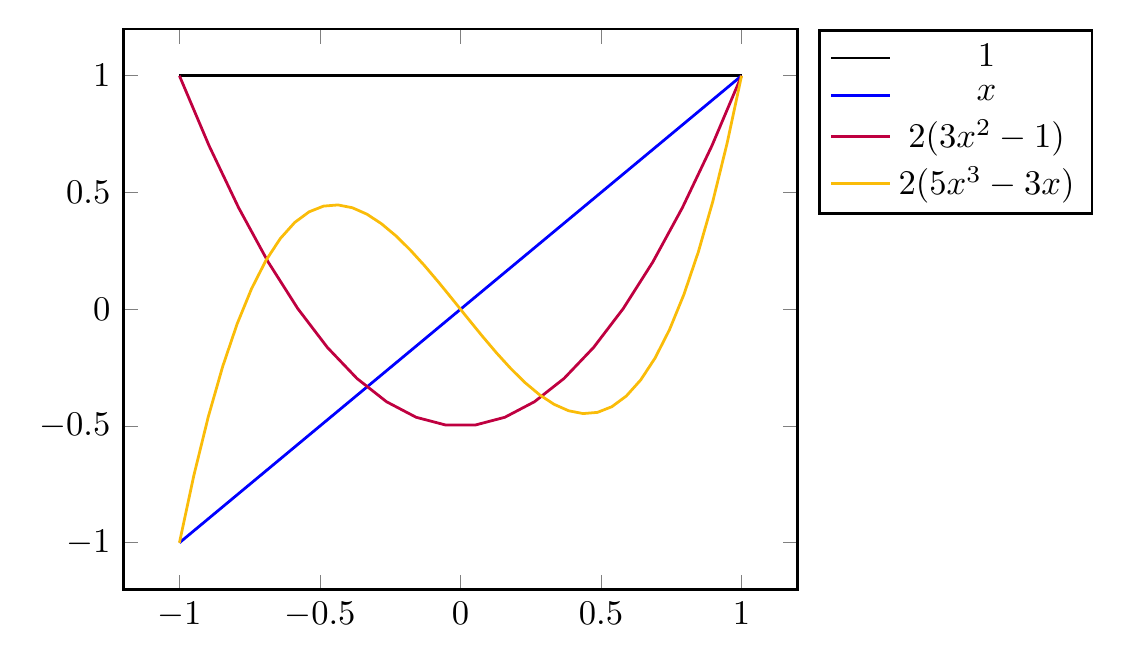
\begin{tikzpicture}[scale=1.25]
                \begin{axis}[range=-1:1,domain=-1:1, thick, legend pos= outer north east]
                    \addplot[samples=2]{1};
                    \addplot[samples=10, blue]{x};
                    \addplot[samples=20, purple]{(3*x^2-1)/2};
                            \addplot[samples=40, yellow!50!orange]{(5*x^3-3*x)/2};
                            \legend{1, 
                            $x$,
                            $\oo{2}\qty(3x^2-1)$,
                            $\oo{2}\qty(5x^3-3x)$}
                \end{axis}
            \end{tikzpicture}
            \caption{The First four Legendre Polynomials ($n=0,1,2,3$)}
            \label{fig:legendre_graph}
        \end{figure}
%\end{document}
\newpage
%\nocite{*} % I didnt cite anything, so I use this to dump all my references here
%\printbibliography{}
\end{document}